\documentclass{standalone}
\usepackage{mathpazo}
\usepackage{tikz}
\usetikzlibrary{calc}
\usetikzlibrary{arrows}

\begin{document}

\def\wat#1#2#3{
\begin{scope}[shift={#1}]
  \node[draw, circle, radius = 0.5] (#2) at (0,0) {#3};
  \draw (#2.north) -- ++(0, 0.5) node[below left] {*}
  -| ($(#2.west) + (-.5,0)$) node[above right] {*}
  -- (#2.west);
\end{scope}
}

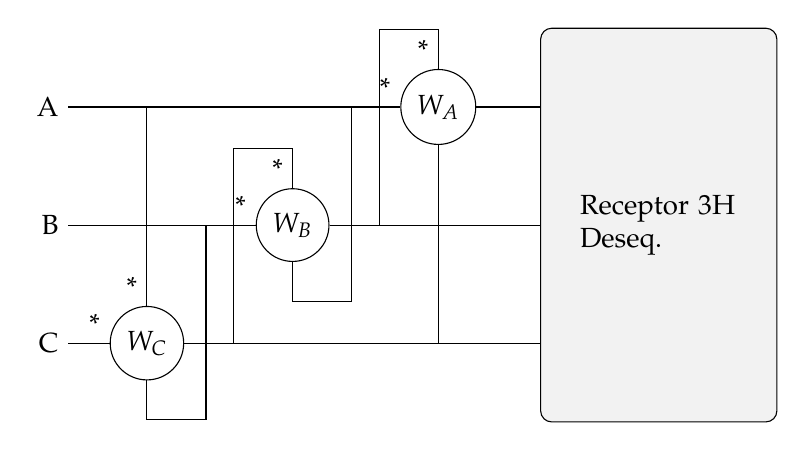
\begin{tikzpicture}
  %% Líneas
  \coordinate (A1) at (-2,4.5);
  \coordinate (A') at ($(A1) + (6, 0)$);
  \coordinate (B1) at ($(A1) + (0, -1.5)$);
  \coordinate (B') at ($(B1) + (6,0)$);
  \coordinate (C1) at ($(B1) + (0, -1.5)$);
  \coordinate (C') at ($(C1) + (6,0)$);
  \coordinate (A2) at ($(A1) + (2, 0)$);
  \coordinate (B2) at ($(A2) + (0, -1.5)$);
  \coordinate (C2) at ($(B2) + (0, -1.5)$);
  \coordinate (A3) at ($(A2) + (2, 0)$);
  \coordinate (B3) at ($(A3) + (0, -1.5)$);
  \coordinate (C3) at ($(B3) + (0, -1.5)$);
  %% vatímetro C
  \node[draw, circle, radius = 0.5] (Wc) at ($(C1) + (1, 0)$) {$W_C$};
  \draw (Wc.north) node[above left] {*};
  \draw (Wc.west) node[above left] {*};
  \draw (Wc.north)  -- ($(A1)!(Wc.north)!(A')$);
  \draw (Wc.south) |- ++(.75, -0.5)
  -- ($(B1)!($(Wc.south) + (.75,0)$)!(B')$);
  %% Salida de corriente de vatímetro
  \draw (Wc.east) -- (C');
  %% Entrada de corriente de vatímetros
  \draw (C1) node[left] {C} -- (Wc.west);
  %% vatímetro B
  \node[draw, circle, radius = 0.5] (Wb) at ($(B1) + (2.85, 0)$) {$W_B$};
  \draw (Wb.north) node[above left] {*};
  \draw (Wb.west) node[above left] {*};
  \draw (Wb.north) |- ++(-.75, 0.5)
  -- ($(C1)!($(Wb.north) + (-.75,0)$)!(C')$);
  \draw (Wb.south) |- ++(.75, -0.5)
  -- ($(A1)!($(Wb.south) + (.75,0)$)!(A')$);
  %% Salida de corriente de vatímetro
  \draw (Wb.east) -- (B');
  %% Entrada de corriente de vatímetros
  \draw (B1) node[left] {B} -- (Wb.west);
  %% vatímetro A
  \node[draw, circle, radius = 0.5] (Wa) at ($(A1) + (4.7, 0)$) {$W_A$};
  \draw (Wa.north) node[above left] {*};
  \draw (Wa.west) node[above left] {*};
  \draw (Wa.north) |- ++(-.75, 0.5)
  -- ($(B1)!($(Wa.north) + (-.75,0)$)!(B')$);
  \draw (Wa.south)  -- ($(C1)!(Wa.south)!(C')$);
  %% Salida de corriente de vatímetro
  \draw (Wa.east) -- (A');
  %% Entrada de corriente de vatímetros
  \draw (A1) node[left] {A} -- (Wa.west);
  %% Receptor
  \draw [rounded corners, fill= gray!10]
  ($(A') + (0, 1)$) rectangle ($(C') + (3,-1)$)
  node[midway, text width = 2cm] {Receptor 3H Deseq.};
\end{tikzpicture}
\end{document}